\scanpage{67}
% archive sheet number: 66
% @ L1–5
c'est qu'il semble que sur la carte $\mathscr X$ obtenue par vrillement, on n'ait aucune interprétation des ``trous'' (ou sommets, quand on a bouché les trous) en termes de la géométrie de $\underline{\Sigma}$.

% @ L6–10
\deleted{\unsure{C}} Il faudrait quand même que je réessaye, pour voir si je \deleted{\unsure{né|ne}} m'étais pas mélangé les pinceaux $\ldots$ \deleted{\unsure{I}} Quand on a fait ce vrillement, et qu'on suit par continuité une orientation choisie

% @ L11–end
$\omega$ de $\Delta_D$ (définie par une or. $\omega_D$ de $D$) en passant de $\Delta_D$ dans $\Delta_{D'}$ via l'arc de transition, on trouve \deleted{que} une orientation $\omega'$ de $\Delta_D$, qui induit sur $D'$ une orientation, $\omega_{D'}$, qui est \uuline{opposée} de celle déduite par transport \deleted{\unsure{de structures}} parallèle ! Voilà donc rectifiée une erreur monumentale, commise dès les débuts !

% @ R1–7
Venons-en à l'autre choix qui donne lieu à $\mathscr X\to X$, savoir $\alpha=a$. On est obligé ici d'ajuster comme j'avais dit $\Delta_D,b$ et $(\Delta_{D'},a)$, pour faire se rencontrer $b$ et $a$ en $b^*\sim a^*\subset X$. On trouve la figure

% @ R, centre
\figure{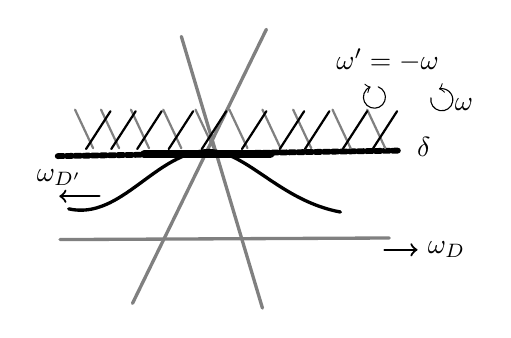
\begin{tikzpicture}[x=1cm,y=1cm,line cap=round]
\draw[very thick,gray] (-.40,1.55)--(.63,-1.9) (.68,1.64)--(-1.02,-1.84);
\draw[very thick,gray] (-1.94,-1.03)--(2.24,-1.01);
\draw[thick,->] (2.18,-1.16)--(2.60,-1.16) node[right] {$\omega_D$};
\draw[very thick] (-1.83,-.64) .. controls (-1.16,-.79) and (-.72,.10) .. (-.04,.10) .. controls (.44,.08) and (.86,-.54) .. (1.62,-.68);
\draw[thick,->] (-1.44,-.48)--(-1.95,-.48) node[above] {$\omega_{D'}$};
\draw[line width=2.1pt,densely dotted] (-1.97,.03)--(2.35,.10);
\draw[line width=3pt] (-.87,.055)--(.73,.055);
\foreach \x in {-1.52,-1.19,-.81,-.4,.01,.44,.86,1.25,1.75,2.19}{\draw[thick,gray] (\x,.13)--++(-.23,.49);}
\foreach \x in {-1.61,-1.29,-.96,-.56,-.14,.37,.85,1.17,1.65,2.03}{\draw[thick] (\x,.12)--++(.31,.48);}
\node at (2.68,.15) {$\delta$};
\draw[->] (2.1,.91) arc (70:-250:.14);
\node at (2.22,1.25) {$\omega'=-\omega$};
\draw[->] (2.77,.77) arc (170:465:.14);
\node at (3.19,.69) {$\omega$};
\end{tikzpicture}}

% @ R, below figure
i.e. on \unsure{vrille|recolle} avec elle-\ensuremath{=} \uline{la $=$ rive} \deleted{de} le long de la ligne critique de spécialisation $\delta$. L'identification $b^*\to a^*$, comme tantôt, est l'iso de transport. Ici, la combinatoire (choix \inserted{d'orien$\unsure{\mathrm t|\mathrm n}$} de structure polygonale sur l'arc de transition associé à une p.v.) est sujette au choix opposé
